\originalsection{摘要}\label{dgm-abstract}
当今多数人工智能系统受到人为设计的固定架构限制，不能自主而持续地改进自身. 相比之下，科学方法是累积性的开放系统，每项创新都建立在此前的成果之上，为未来发现创造条件. 人们越来越希望，当前依赖人工推动人工智能进步的过程本身也能实现自动化. 如果能够安全地完成，这种自动化将加速人工智能的发展，让我们更早获得其益处. 这一前景提出了一个问题：人工智能系统如何在不断提高相关问题求解能力的同时，无休止地改进自身？元学习能够自动发现新算法，但受限于一阶改进，以及人为设计的合适搜索空间. 哥德尔机\cite{dgm-schmidhuber2007godel}提出了一种理论替代方案：一种反复修改自身、且每次修改都可证明有益的自我改进人工智能. 遗憾的是，在实践中证明多数修改具有净收益是不可能的. 我们提出达尔文哥德尔机（Darwin Gödel Machine，DGM），一种新的自我改进系统；它迭代修改自己的代码，由此也改进修改自身代码库的能力，并用编码基准对每次变化进行经验验证. 受达尔文演化和开放式研究启发，DGM 逐步扩大生成的编码智能体档案. 它从档案中抽取智能体，这些智能体通过自我修改产生新的、有趣的版本. 这种开放式探索形成一棵不断生长的、多样且高质量的智能体树，并支持并行探索搜索空间中的多条不同路径. 实验中，DGM 自动改进其编码能力，例如获得更好的代码编辑工具、长上下文窗口管理和同行评审机制，使 SWE-bench 的表现从 20.0\% 提高到 50.0\%，Polyglot 从 14.2\% 提高到 30.7\%. 此外，DGM 显著优于不具备自我改进或开放式探索的基线. 所有实验均采取安全防护，如沙箱和人工监督. 总体而言，DGM 朝着自我改进人工智能迈出了重要一步，能够沿着通向无尽创新的路径收集自己的垫脚石. 全部代码开源于 \url{https://github.com/jennyzzt/dgm}.

\originalsection{1 引言}\paperlabel{1}{dgm-sec:intro}
科学进步具有累积性与开放性，每次突破都建立在无数先前认识之上. 同样，最先进的人工智能系统也建立在悠久的创新谱系上. 例如，当今大语言模型\cite{dgm-brown2020language}的骨干 Transformer\cite{dgm-vaswani2017attention}并非凭空出现，而是建立在多年的先前创新上，包括循环神经网络\cite{dgm-linnainmaa1970representation,dgm-amari1972learning,dgm-hopfield1982neural,dgm-rumelhart1985learning}和注意力机制\cite{dgm-schmidhuber1990learning,dgm-bahdanau2015neural,dgm-kim2017structured,dgm-parikh2016decomposable}. 然而，当今多数系统仍受人为设计的固定架构约束，只能在预设边界内学习，不能自主重写自身源码来改进自己. 因此，人工智能发展的每项进步仍高度依赖人为干预，牵制了进步的速度. 本文研究一种令人关注的可能性：安全地自动搜索越来越好的人工智能. 可以设想，人工智能系统像科学发现本身一样，成为自身发展的动力：建立在过去成果上，递归改进，推动自己获得更先进的能力.

\begin{figure}[ht]
\centering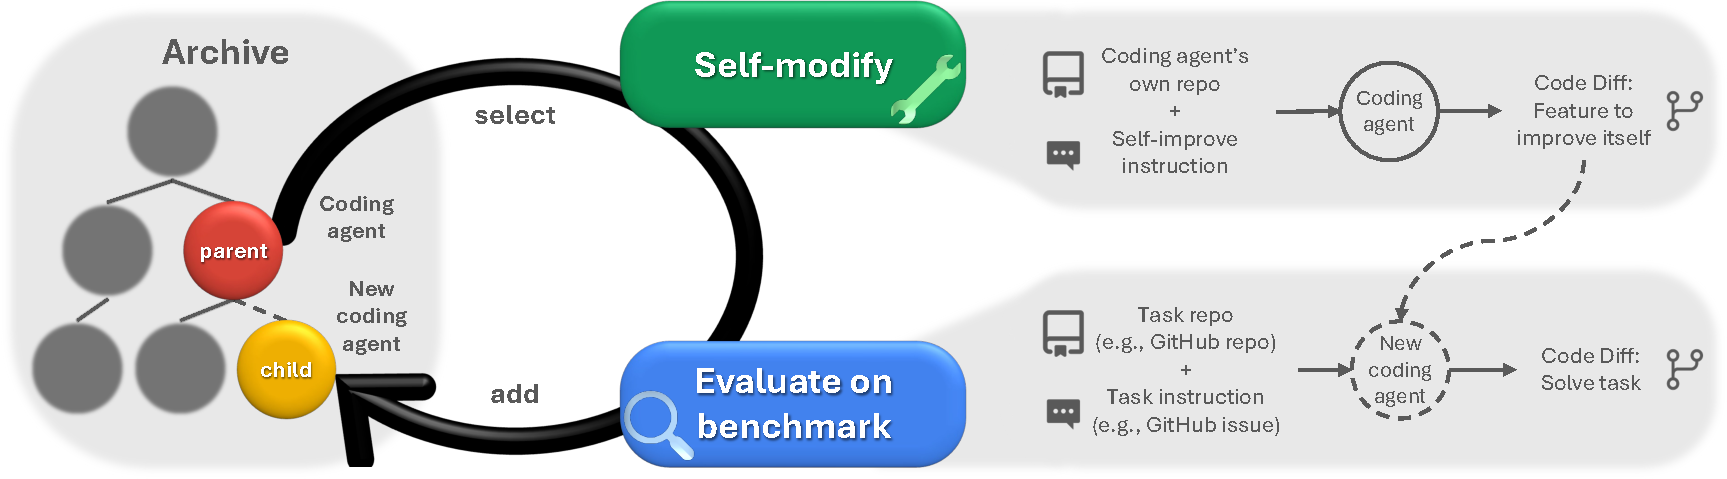
\includegraphics[width=.94\textwidth]{../papers/translations/dgm/figures/conceptual.pdf}
\caption{达尔文哥德尔机. DGM 交替执行自我修改与下游任务评价，迭代构建不断扩大的智能体档案. 通过开放式探索，选择档案中的智能体执行自我修改. 原图：Jenny Zhang、Shengran Hu、Cong Lu、Robert Lange、Jeff Clune，CC BY 4.0；图内英文标注保留.}\label{dgm-fig:conceptual}
\end{figure}

Schmidhuber\cite{dgm-schmidhuber2007godel}提出了一类具有严格数学基础的、自指的、自我改进问题求解器. 它依赖形式证明来论证代码重写，确保任何自我修改都可证明有益. 但在实践中，如果不对系统作限制性假设，就无法形式证明对人工智能系统的一项修改是否有益. 例如，看似给基于大语言模型的编码智能体更多工具——代码搜索、测试运行器等——会带来益处，但实际影响高度依赖模型训练和任务上下文；针对一种设置优化的测试工具，可能在另一种设置下让智能体困惑. 我们不要求形式证明，而是根据基准经验验证自我修改，使系统能依据观测结果改进和探索. 这类似生物演化：突变和适应并不事先得到验证，而是在产生、试验之后经自然选择保留. 我们也从达尔文演化\cite{dgm-darwin2023origin}获得启发，研究保留此前发现的智能体库、让其成为后代垫脚石的有效性.

我们提出\textbf{达尔文哥德尔机（DGM）}，一种自指、自我改进系统，通过编写和修改自己的代码成为更好的编码智能体. 每次自我修改都要求 DGM 编辑自己的代码库. 我们使用图灵完备的 Python，因此 DGM 在潜力上能够构建任何可计算机器. 我们的框架设想智能体可以重写自己的训练脚本，包括训练新的基础模型（FM）. 但本文没有展示这一点，因为训练基础模型计算量很大，会引入大量额外复杂性，我们将其留作未来工作. 本文聚焦于使用冻结预训练基础模型的编码智能体设计改进，如工具使用与工作流. DGM 交替执行自我修改和评价. 自我修改阶段，从档案中选出的编码智能体生成自己的修改版本；评价阶段，对每个修改后的智能体进行编码基准测试，估计其编码能力，再加入档案. 通过这一循环改善能力后，DGM 在解决编码任务和进行未来自我改进方面都变得更好. 一个关键假设是，编码基准表现提高意味着编码能力更好，从而自我修改与自我改进能力也更好. 此外，DGM 维护生成智能体的档案，从一个智能体开始，随时间持续积累全部变体. 为支持持续自我改进，DGM 借鉴开放式研究\cite{dgm-wang2019paired,dgm-fernandopromptbreeder,dgm-faldor2025omni}，积累多样的垫脚石，即有趣但次优、可能促成未来突破的解或特征. 开放式探索鼓励发现超出即时性能收益的新颖且可能有用的自我修改.

我们在两个编码基准 SWE-bench\cite{dgm-jimenez2024swebench}与 Polyglot\cite{dgm-gauthier2024polyglot}上报告结果. DGM 在 SWE-bench 上从 20.0\% 自动提高到 50.0\%，在 Polyglot 上从 14.2\% 提高到 30.7\%. 我们表明，自我改进支持持续进步：DGM 优于始终用同一个基础智能体修改并生成新智能体、却不进行自我改进的基线. 我们还表明，开放式探索与保留全部此前生成智能体的档案，有助于发现更好的编码智能体. DGM 优于不进行开放式探索的基线；后者不积累有趣且彼此不同的垫脚石档案，编码智能体始终建立在自身最新版本上. 总体而言，DGM 朝着能积累先前创新并递归改进的人工智能系统迈出了一步. 我们广泛讨论安全问题，包括沙箱化和自我修改的可追溯性，以保证负责任的实验（见\ref{dgm-sec:safety}节）. 推进安全、自指、自我改进模型的可能性，使我们更接近不仅会学习、还会像科学一样沿开放式、自加速轨迹演化的人工智能.

\originalsection{2 相关工作}\paperlabel{2}{dgm-sec:related}
\textbf{开放式.} 推动无界创新的一项重大挑战，是设计不断生成新颖且可学习成果的开放式人工智能系统\cite{dgm-stanley2017open}. Hughes 等\cite{dgm-hughes2024open}把开放式刻画为系统从观察者视角生成既新颖又可学习的成果序列的能力. 核心困难是如何组织和探索庞大搜索空间，持续产生对人有趣的成果\cite{dgm-clune2019ai,dgm-jiang2023general}. 早期进展来自质量多样性算法、目标导向探索、内在动机和学习进度框架\cite{dgm-pugh2016quality,dgm-ecoffet2019go,dgm-lehman2011novelty,dgm-oudeyer2007intrinsic}；近期进展则用大规模基础模型作为人类趣味的代理，并作为跨领域生成和评价新行为的通用引擎\cite{dgm-brown2020language,dgm-hu2025automated,dgm-zhang2024omni}. 但这些方法尚未闭合自指自我改进循环，即下游任务改进还未转化为更强的自我修改能力或进一步创新的加速. 我们希望模拟科学技术的加速过程，新工具和发现会催生更多发现. 如何模仿自然的演化轨迹，使其不仅朝复杂性发展，还朝着越来越强的演化能力发展\cite{dgm-dawkins2019evolution,dgm-gerhart2007theory,dgm-hendrikse2007evolvability}？

\textbf{基础模型智能体的元学习.} 许多基于基础模型的智能体由人工设计. 构建模块包括提示工程\cite{dgm-chen2023unleashing,dgm-schulhoff2024prompt}、思维链\cite{dgm-wei2022chain,dgm-yao2023react,dgm-hu2023ThoughtCloning,dgm-guo2025deepseek,dgm-lightman2023let,dgm-muennighoff2025s1,dgm-zelikman2024quiet}、自我反思\cite{dgm-shinn2023reflexion,dgm-yao2023react,dgm-madaan2303self}、多智能体辩论\cite{dgm-zhuge2023mindstorms,dgm-liang2023encouraging,dgm-khan2024debating}、记忆\cite{dgm-liu2023think,dgm-zhong2024memorybank,dgm-modarressi2023ret}、温度采样\cite{dgm-zhu2024hot}与检索增强生成\cite{dgm-lewis2020retrieval}. 人工组合这些模块，会让系统能力受限于设计者的创造力. 近期出现的元学习方法使用基础模型自动优化提示\cite{dgm-fernandopromptbreeder,dgm-meta2022human,dgm-khattab2023dspy,dgm-cheng2025trace,dgm-yuksekgonul2024textgrad,dgm-yuan2024evoagent}和设计智能体模块\cite{dgm-zhang2024aflow,dgm-zhou2024symbolic,dgm-yin2024g,dgm-zhugegptswarm,dgm-rosser2025agentbreeder,dgm-zhang2025multi,dgm-ye2025mas,dgm-gao2025flowreasoner,dgm-nie2025weak,dgm-su2025debflow,dgm-zhang2025gnns,dgm-niu2025flow}. 智能体系统的自动化设计（ADAS）\cite{dgm-hu2025automated}用固定的元智能体迭代生成下游智能体，在目标基准上评价，并利用反馈改进后续生成. 相比之下，DGM 是单一系统，既解决下游编码问题，又改进自己的实现即代码库，不再需要固定、人工设计的元智能体，从而支持自指改进.

\textbf{自我改进人工智能.} 早期研究者提出了自我改进的理论和概念方案\cite{dgm-good1966speculations,dgm-schmidhuber1987evolutionary,dgm-schmidhuber2007godel}. 一些实践方法包括以神经网络权重参数化定义的系统\cite{dgm-schmidhuber1993self,dgm-hall2007self,dgm-hobbhahn2025swebenchmini,dgm-kirsch2022self,dgm-irie2022modern,dgm-irie2025metalearning,dgm-lu2023arbitrary,dgm-havrilla2024glore}. Metz 等\cite{dgm-metz2021training}开发了一个基于梯度的优化器，利用种群训练\cite{dgm-jaderberg2017population}的变体进行自指元训练. Lange 等\cite{dgm-lange2023discovering}把这种方案扩展到无梯度学习. Silver 等\cite{dgm-silver2017mastering}利用自博弈持续演化智能体，在国际象棋与围棋等困难领域取得超人表现. 更接近 DGM 的是近期使用基础模型智能体进行自我改进的方案\cite{dgm-yin2024g,dgm-robeyns2025self,dgm-hu2024self,dgm-zelikman2024self,dgm-huang2022large,dgm-singh2023beyond}. Zelikman 等\cite{dgm-zelikman2024self}用元智能体生成下游智能体，再依据生成解的元效用更新元智能体. Yin 等\cite{dgm-yin2024g}用同一个系统解决下游任务并递归修改自身. 但下游任务或元效用并不总与自我改进所需能力一致. 在 DGM 中，下游任务提升直接反映自我改进能力增强，因此具有自加速进步的潜力. 最相似的同期工作是 Robeyns 等\cite{dgm-robeyns2025self}，它也让单一智能体递归解决编码问题并修改自己的代码库. 与该工作以及 Zelikman 等、Yin 等的主要区别在于，DGM 具有开放式探索循环，鼓励超越即时收益的自我修改，避免在次优状态停滞. 附录\hyperref[dgm-app:related]{B}还讨论程序合成与达尔文演化的相关工作.

\originalsection{3 达尔文哥德尔机}\paperlabel{3}{dgm-sec:methods}
哥德尔机是一种理论构想：寻找可证明能改进自身的方法的人工智能\cite{dgm-schmidhuber2007godel}. 本文提出 DGM，尝试实现创造哥德尔机的长期梦想. DGM 放宽了哥德尔机不切实际的要求，即从理论上证明一项变化能改善系统；它改为要求通过实验中的经验证据，展示所提议的新版本提升了表现. 此外，依赖改进的经验证据，可能让 DGM 陷入全部可计算算法这一庞大可能系统空间的局部最优. 为此，DGM 在搜索中维护已发现解的档案，支持开放式探索，而不只演化一个解. 这些原则呼应达尔文演化\cite{dgm-darwin2023origin}（附录\hyperref[dgm-app:related]{B}）：从此前发现解的档案选出实体、修改它，并在它以有趣方式变新时保留\cite{dgm-zhang2024omni,dgm-faldor2025omni,dgm-stanley2015greatness}. 因此我们把算法称为达尔文哥德尔机（图\ref{dgm-fig:conceptual}）.

\textbf{编码智能体的自指自我改进.} DGM 仅以一个编码智能体初始化，并用编码基准评价进展. 编码智能体定义为一个以代码仓库实现、由冻结预训练基础模型驱动、能读写和执行代码的单一系统. 用 Python 等通用图灵完备语言表达的代码，是构建与改进智能系统的强大媒介，因为它可以表示任何可计算过程. 近期工作\cite{dgm-hu2025automated,dgm-zhang2024aflow}表明，可以通过对代码仓库中实现的提示、工作流与工具等设计进行元学习来改进智能体. 因而，我们把自我改进定义为修改智能体自身模块设计、也就是自身代码的一项编码任务；不包含下一段的开放式探索过程. 关键动机在于，经验证据必须同时反映系统自我改进和解决下游任务的能力. 把 DGM 配置为编码智能体并测试编码能力，观察到的改进不仅展示下游表现增强，也展示进一步自我改进的能力，因为自我改进本质上是一项修改编码智能体自身代码仓库的编码任务.

\textbf{基于种群的开放式探索.} DGM 从一个初始编码智能体开始，建立全部已发现智能体的档案. 每次迭代选出父智能体，让其自我修改并分支产生新智能体. 父代选择大体正比于各智能体的表现分数，反比于具有代码库编辑功能的子代数（附录\hyperref[dgm-app:parent-select]{C.2}）. 这偏向表现良好而探索不足、即现有子代较少的智能体，兼顾利用强表现者与探索有希望但采样较少的谱系. 每个智能体保留非零选择概率，确保在计算资源足够时任何改进路径仍有可能. 每个被选父代分析自己的基准评价日志，提出下一项待实现功能，再把提案作为问题描述执行（附录\hyperref[dgm-app:selfimprove-prompts]{C.3}）. 父代将建议功能实现在自身代码库中，生成新编码智能体. 每个新智能体在选定编码基准上被定量评价，估计其编码能力. 只有成功编译且仍能编辑指定代码库的智能体才加入档案，因为只有它们能继续自我修改，其余均被丢弃. 父代选择、自我修改与评价循环不断进行，逐步扩充解的档案. 重要的是，归档的解可能成为在很久之后才带来改进的垫脚石，因此本方法与爬山式智能体设计\cite{dgm-robeyns2025self}有实质区别. 当前开放式探索过程，即档案维护与父代选择，是固定的，不能由 DGM 修改；我们将其留作未来方向. 附录\hyperref[dgm-app:pseudocode]{C.4}给出算法伪代码.

\originalsection{4 实验}\paperlabel{4}{dgm-sec:experiments}
第\ref{dgm-sec:experiment-setup}节介绍包括初始编码智能体在内的实验设置. 我们在 SWE-bench\cite{dgm-jimenez2024swebench}和 Polyglot\cite{dgm-gauthier2024polyglot}上实验（第\ref{dgm-sec:benchmarks}节）. 每个基准均比较 DGM 与两个基线：无自我改进智能体的 DGM、无开放式探索的 DGM（第\ref{dgm-sec:baselines}节）. 所有实验中 DGM 都优于两个基线，表明自我改进机制与开放式探索对持续性能增益至关重要（第\ref{dgm-sec:results}节）. 我们还展示所发现特征能跨模型、基准和任务迁移.

\originalsection{4.1 实验设置}\paperlabel{4.1}{dgm-sec:experiment-setup}
DGM 以单一编码智能体初始化. 基础智能体围绕冻结基础模型构建，增加工具使用能力\cite{dgm-schick2023toolformer,dgm-anthropic_tool_use_2024}. 基础模型自主决定每一步的动作，使用它认为适合的工具. 基础智能体有两个工具：执行 bash 命令的 Bash 工具，以及查看和编辑目录、整个文件的编辑工具（附录\hyperref[dgm-app:initial-agent]{C.1}）. 智能体收到一个输入提示，说明目标仓库位置、问题描述和仓库测试框架. 我们故意让基础智能体保持轻量，提供可清楚展示自我改进的简单起点. DGM 运行 80 次迭代，每次生成一个新智能体；SWE-bench 同时运行两次迭代，Polyglot 同时运行四次（附录\hyperref[dgm-app:parent-select]{C.2}）. 两个基准中的自我修改均由 Claude 3.5 Sonnet（New）\cite{dgm-anthropic2024claude35sonnet}驱动. 基准评价时，SWE-bench 使用 Claude 3.5 Sonnet（New），Polyglot 使用 o3-mini\cite{dgm-openai2025o3mini}（附录\hyperref[dgm-app:fm-hyperparam]{D.1}）.

\originalsection{4.2 基准}\paperlabel{4.2}{dgm-sec:benchmarks}
我们在两个流行编码基准上评价 DGM；它们考察编码任务的不同方面，从而验证算法在不同用例中的有效性. SWE-bench 与 Polyglot 均评价人工智能智能体自动解决编码任务的能力. 给定代码仓库和任务指令，智能体需修改仓库以完成任务. 二者均被广泛使用\cite{dgm-zhang2024autocoderover,dgm-zhang2024rest,dgm-xia2024agentless,dgm-cao2024spider2,dgm-GoogleDeepMind2025GeminiThinking,dgm-aider2024}，要求智能体浏览仓库、理解不同文件中函数的关联，在复杂代码里识别细小错误. SWE-bench 只有 Python 任务，Polyglot 涵盖多种语言. 另一个区别是，SWE-bench 任务可能需编辑多个文件，而 Polyglot 主要需在单个文件从头实现解法；尽管仍需查看其他文件来理解必要修改，但总体编辑文件数更少.

\textbf{SWE-bench.} 为避免在不可解任务上浪费计算，我们使用 SWE-bench Verified\cite{dgm-openai2024sweverified}，即经人工筛选、所有任务均可解的 SWE-bench\cite{dgm-jimenez2024swebench}子集. 本文的 SWE-bench 默认指这一 Verified 子集.

\textbf{Polyglot.} Polyglot 包含 C++、Rust、Python 等多种编程语言任务\cite{dgm-gauthier2024polyglot}. 相比最常用且可能已包含于基础模型训练集的 SWE-bench，Polyglot 更小众，更不可能包含于基础模型后训练数据. 此外，Polyglot 主要由其开发者用于评价 Aider\cite{dgm-aider2024}. 这提供了比较自动设计智能体与社区代表性编码智能体的机会，后者由人类开发者持续开发，并针对 Polyglot 测试超过一年. Polyglot 还允许检验 DGM 超出 Python、泛化到多语言的能力. 我们遵循 Polyglot 排行榜设置，但有一项关键区别：排行榜报告 pass@2，允许智能体查看一次真实测试反馈；我们报告 pass@1，智能体从不看到真实测试结果.

完整基准评价昂贵（附录\hyperref[dgm-app:cost-estimate]{E.1}），我们因此采用分阶段评价来估计编码表现. 一般而言，越确信某智能体相对强，就用更多任务评价它. 先在 10 项任务上验证基本代码库编辑功能. 只有仍能编辑代码的智能体，才可解决下游编码任务或继续自我修改. 通过初始阶段后，再在扩展的 50 项任务上评价. SWE-bench 任务依据 SWE-bench-verified-mini\cite{dgm-hobbhahn2025swebenchmini}选择，后者旨在代表完整基准（附录\hyperref[dgm-app:swebench-tasks]{E.2}）；Polyglot 任务为完整基准的随机子集（附录\hyperref[dgm-app:polyglot-tasks]{E.3}）. 所用大语言模型固有的随机性会造成表现噪声. 较小子集用于估计总体有效性、识别优良候选. SWE-bench 中，若智能体在 60 任务子集上成功率超过 40\%，且排在档案前两名，就再在 200 个任务上评价，即原 60 个加 140 个，以更精确衡量真实编码能力；40\% 是依据预运行噪声选择的启发式阈值. Polyglot 中，若在 10 任务子集上成功率超过 40\%，则在扩展的 50 任务子集上评价.

\originalsection{4.3 基线}\paperlabel{4.3}{dgm-sec:baselines}
为隔离 DGM 核心组件的贡献，我们比较\textbf{无自我改进的 DGM}与\textbf{无开放式探索的 DGM}. 前者在此设置下复现 ADAS\cite{dgm-hu2025automated}的方法：负责修改编码智能体的元智能体在整个实验中始终固定为基础智能体（原文算法 2）. 这用于考察迭代自我改进在加速更好编码智能体演化中的作用. 后者移除档案，始终修改最新保存的自身版本（原文算法 3）. 若智能体自我修改到丧失编辑代码库所需的基本功能，就无法继续修改自身或解决任何编码任务；因而该基线保留仍维持基本编辑功能的最新版本. 它用于评价档案以及已有充分记录的开放式探索有益原则\cite{dgm-clune2019ai,dgm-stanley2015greatness,dgm-zhang2024omni,dgm-fernandopromptbreeder,dgm-lee2020learning,dgm-samvelyan2024rainbow,dgm-colas2022autotelic}对智能体演化的作用.

除学习型基线外，我们还比较人工设计的开源方案. SWE-bench 采用经核验、即 SWE-bench 团队能复现结果的最佳开源方案（附录\hyperref[dgm-app:swebench-sota]{E.4}）. Polyglot 采用代表性智能体 Aider\cite{dgm-aider2024}，它开源且设计为支持多语言和大型代码库编辑（附录\hyperref[dgm-app:polyglot-sota]{E.5}）. 为公平比较，在评价 DGM 的相同任务子集上测量解题比例；图\ref{dgm-fig:dgm-comparisons}中的水平虚线展示这些值.

\originalsection{4.4 结果}\paperlabel{4.4}{dgm-sec:results}
\begin{figure}[ht]
\centering
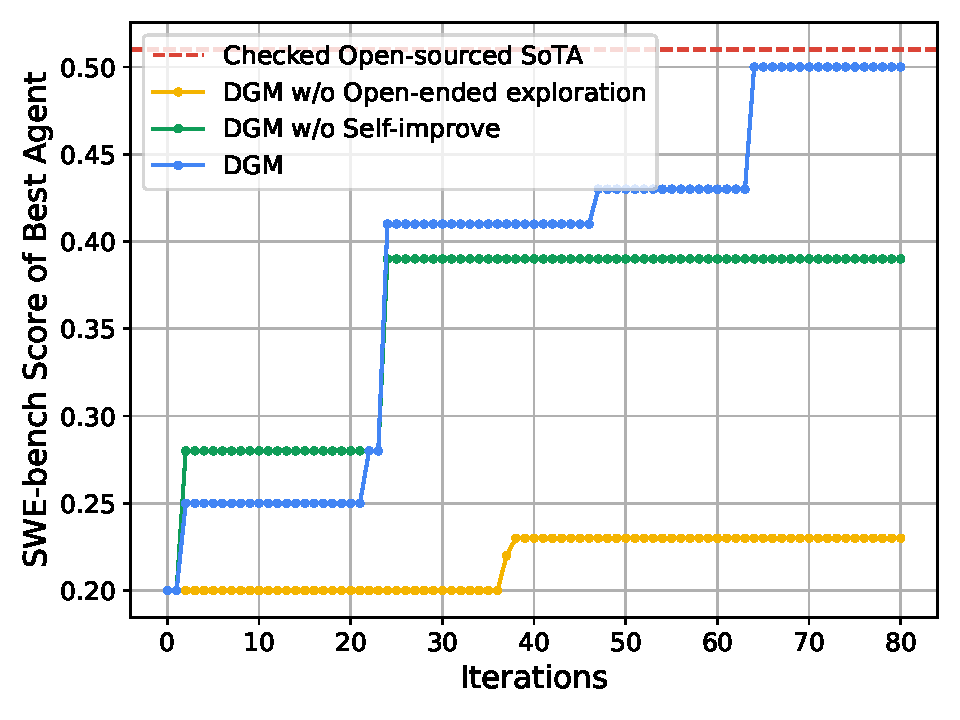
\includegraphics[width=.47\textwidth]{../papers/translations/dgm/figures/dgm_comparisons.pdf}\label{dgm-fig:dgm-comparisons-swe}
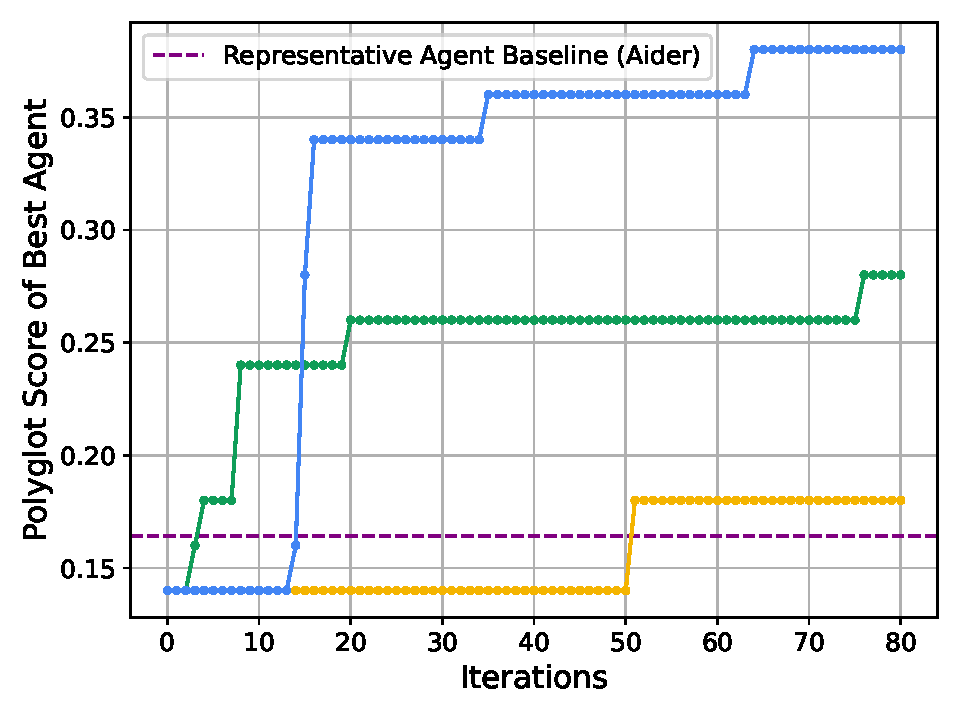
\includegraphics[width=.47\textwidth]{../papers/translations/dgm/figures/dgm_comparisons_polyglot.pdf}\label{dgm-fig:dgm-comparisons-polyglot}
\caption{自我改进与开放式探索使 DGM 持续进步并改善表现. DGM 自动发现越来越好的编码智能体，在左侧 SWE-bench 与右侧 Polyglot 上均取得更好表现. 它优于缺少自我改进或开放式探索的基线，表明两个组件对持续自我改进都至关重要. 分数来自第\ref{dgm-sec:benchmarks}节所述基准子集. 原图：Jenny Zhang、Shengran Hu、Cong Lu、Robert Lange、Jeff Clune，CC BY 4.0；英文标注保留.}\label{dgm-fig:dgm-comparisons}
\end{figure}
\begin{figure}[ht]
\centering
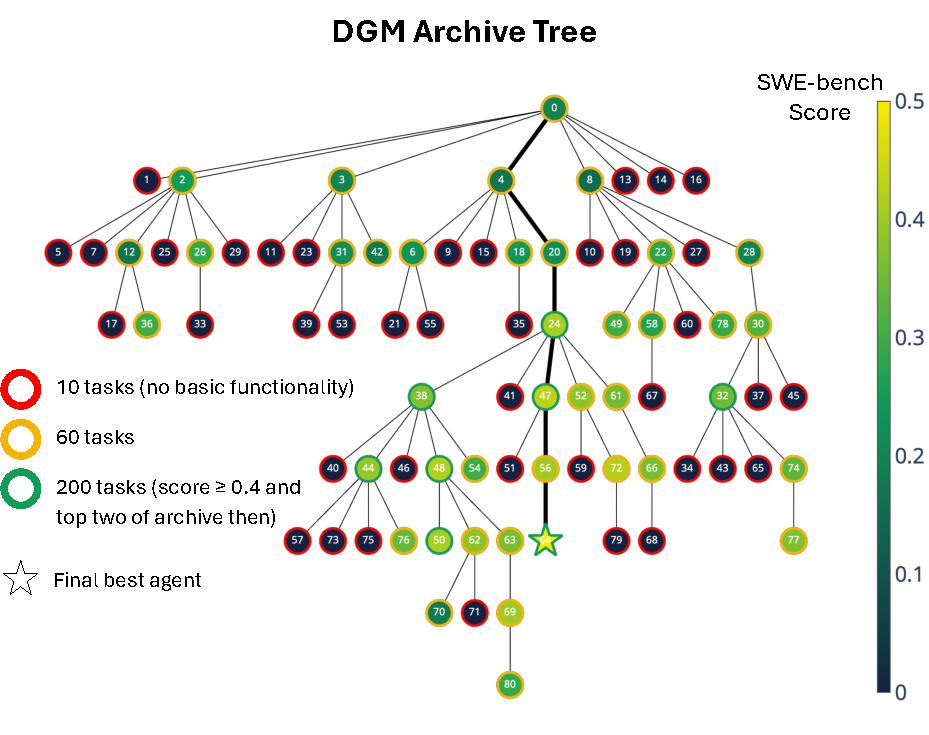
\includegraphics[width=.47\textwidth]{../papers/translations/dgm/figures/dgm_archive.pdf}
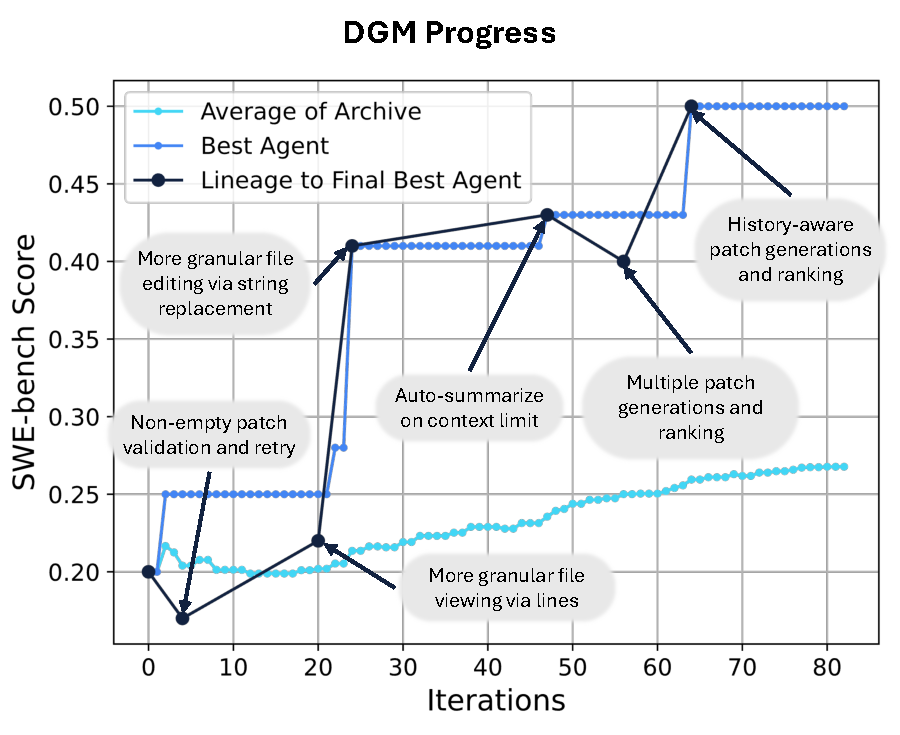
\includegraphics[width=.47\textwidth]{../papers/translations/dgm/figures/dgm_progress.pdf}
\caption{DGM 自动自我改进，成为更好的编码智能体. 左：SWE-bench 运行中生成的智能体档案. 每个节点代表一个编码智能体，节点 0 是基础智能体. 节点颜色表示 SWE-bench 表现即解题百分比，边框颜色表示该智能体评价过的任务数. 边表示哪个智能体自我修改产生了子代. 许多创新路径经过表现较差的节点，而节点 24 等关键创新引发建立于其上的创新爆发；这两点都体现开放式搜索的益处. 右：SWE-bench 上的 DGM 进展图. 浅蓝线是全部具有基本代码库编辑功能智能体的平均分，蓝线是每次迭代时档案中任一智能体达到的最高分，深色线是最终最佳智能体及其前驱的谱系，其中有两次性能下降. 这展示开放式搜索的益处：探索多样且有趣的垫脚石，而非只从当前最好解分支. 原图：Jenny Zhang、Shengran Hu、Cong Lu、Robert Lange、Jeff Clune，CC BY 4.0；英文标注保留.}\label{dgm-fig:dgm-archive}\label{dgm-fig:dgm-progress}
\end{figure}

80 次迭代后，编码智能体在 SWE-bench 上从 20.0\% 提高到 50.0\%，在 Polyglot 上从 14.0\% 提高到 38.0\%（图\ref{dgm-fig:dgm-comparisons}）. 因 Polyglot 实验设置仅评价 50 项任务，我们另在完整 Polyglot 基准上评价基础智能体和 DGM 发现的最佳智能体，以更精确估计改进；完整基准上从 14.2\% 提高到 30.7\%. 这表明 DGM 能自动自我改进，生成更好的编码智能体. 此外，所发现最佳智能体的表现可比于 SWE-bench 经核验、开源、人工设计的最佳方案. Polyglot 中，尽管基础智能体表现低于 Aider，DGM 仍发现了远超 Aider 的智能体. 两个基准中，发现的智能体可比于或优于人工设计智能体. SWE-bench 最佳智能体与 Aider 都经过人类精心塑造，而 DGM 提示了这样的未来：这种创造力可以自动化，通过持续自我改进的自指循环不断演化.

DGM 自动改善工具与基础模型的使用工作流（图\ref{dgm-fig:dgm-progress}）. 例如，它把编辑工具改为支持按行查看文件、通过字符串替换精确编辑，而非总是查看或替换整个文件. 工作流改进包括多次尝试解题，用另一基础模型评价并选出最好方案，以及生成后续尝试时考虑此前尝试. 附录\hyperref[dgm-app:best-agent-dgm]{F.1}与\hyperref[dgm-app:best-agent-dgm-polyglot]{F.2}分别展示通往两个基准最终最佳智能体的全部修改.

开放式探索允许以非零概率从档案中任何智能体分支，因此 DGM 能摆脱具有误导性的性能低谷或高峰. 例如 SWE-bench 的第 4 与 56 次迭代中，虽然智能体分数暂时低于父代，DGM 仍沿该路径探索创新，产生超过全部前驱的新智能体. 此外，开放式探索允许尝试相同目标功能的不同实现. 例如，更精细编辑工具的具体实现可以有很大差异，导致显著不同的表现（附录\hyperref[dgm-app:supp-dgm-diffimpl]{G}）. DGM 可以探索多个实现，寻找更适合的方案，而不陷入次优实现.

DGM 在两个基准上均优于无自我改进和无开放式探索的基线. 不更新负责修改编码智能体的元智能体时，无自我改进基线在初期提升智能体，但增益很快趋缓（附录\hyperref[dgm-app:plots-swe]{A.1}）. 无开放式探索基线只保留最近的智能体，因此表现差的自我修改会增加后续改进难度.

\begin{figure}[ht]
\centering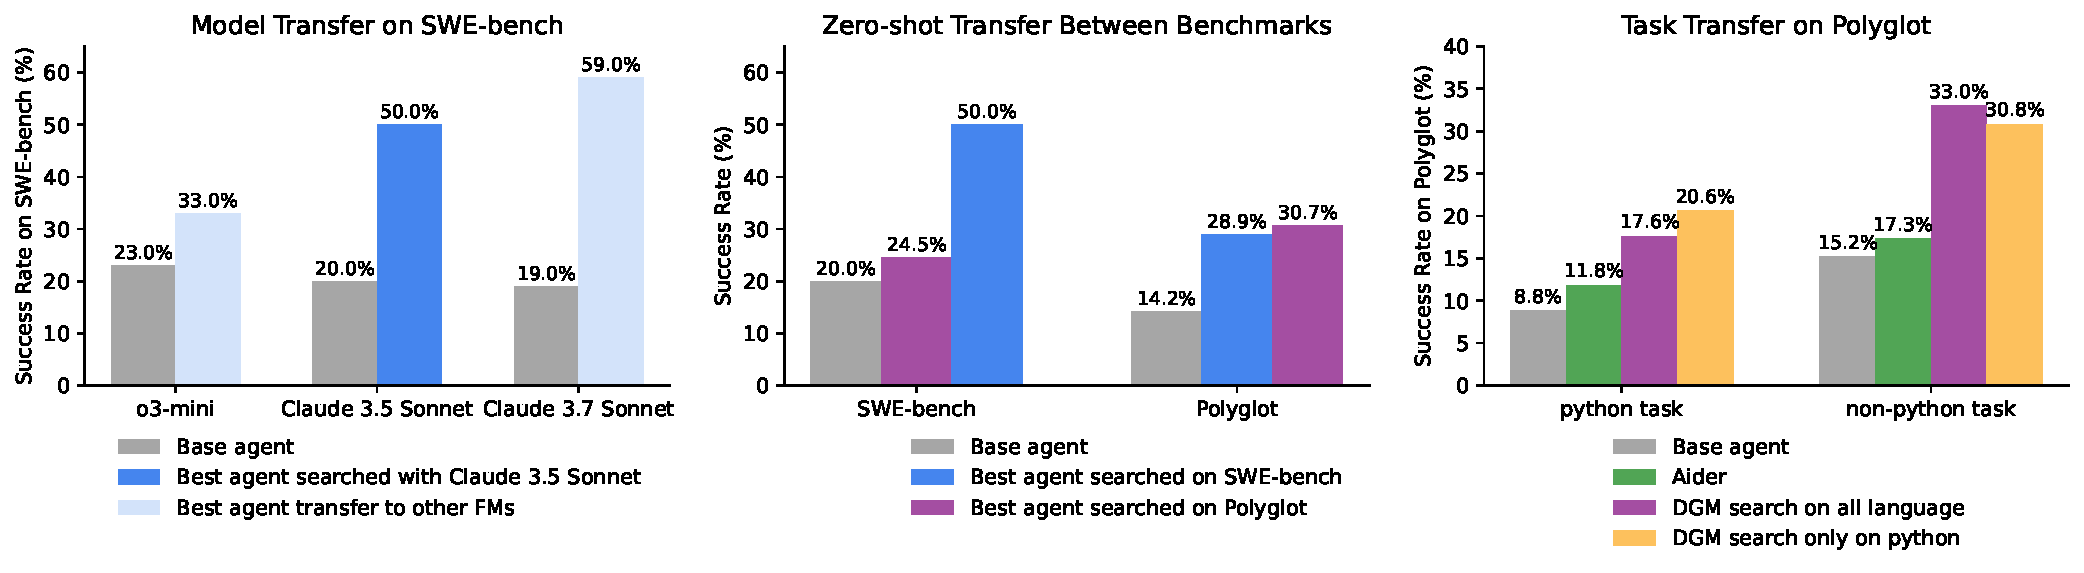
\includegraphics[width=.94\textwidth]{../papers/translations/dgm/figures/transfer_model_task.pdf}
\caption{模型、基准与任务间的迁移. DGM 发现智能体的更好表现可以迁移到不同模型（左）、不同基准（中），以及 Polyglot 中不同编程语言的任务（右），例如从 Python 任务迁移到 C++ 任务. 原图：Jenny Zhang、Shengran Hu、Cong Lu、Robert Lange、Jeff Clune，CC BY 4.0；英文标注保留.}\label{dgm-fig:transfer-overview}
\end{figure}

为评价改进的普遍性，我们用不同于优化时使用的基础模型测试基础智能体与运行中发现的最佳智能体. SWE-bench 运行使用 Claude 3.5 Sonnet（New），迁移评价把模型替换为 Claude 3.7 Sonnet\cite{dgm-anthropic2025claude37}或 o3-mini，在 200 个任务上评价（图\ref{dgm-fig:transfer-overview}左）. 使用 o3-mini 时，基础智能体 23.0\%，发现智能体 33.0\%；使用 Claude 3.7 Sonnet 时，分别为 19.0\% 与 59.5\%. 这提示改进可跨基础模型泛化，而非紧密耦合于运行时使用的特定模型. Polyglot 模型迁移结果见附录\hyperref[dgm-app:polyglot-model]{A.2}.

我们进一步研究跨基准和编程语言迁移. 首先，把在一个基准如 SWE-bench 上发现的最佳智能体用于完全留出的另一基准如 Polyglot，反向亦然（图\ref{dgm-fig:transfer-overview}中）. SWE-bench 演化出的最佳智能体在 Polyglot 达到 28.9\%，初始基线是 14.2\%；Polyglot 演化出的最佳智能体在 SWE-bench 达到 24.5\%，原基线是 20.0\%. 每个智能体优化时从未访问另一基准，因此这些评价是真正的留出测试. 跨基准一致的增益支持我们关于改进反映通用技能获得、而非过拟合或利用基准特定痕迹的论断. 其次，我们用只在 Polyglot 的 Python 任务上训练的 DGM，再把发现智能体迁移到其他语言. 与全语言训练相比，聚焦 Python 稍微改善 Python 表现，但降低非 Python 表现（图右）. 然而，从 Python 迁移到搜索时未见的语言后，智能体仍达到可比于全语言 DGM 的表现，显著优于基础智能体与 Aider. 这些结果展示改进的稳健性，说明并未过拟合于某一语言. 附录\hyperref[dgm-app:add-results]{A}给出更多结果.

\originalsection{5 安全讨论}\paperlabel{5}{dgm-sec:safety}
DGM 等自我改进系统朝更自主的人工智能开发迈出一步，符合构建能造福人类的强人工智能这一长期目标\cite{dgm-schmidhuber1987evolutionary,dgm-clune2019ai,dgm-markoff2016machines,dgm-lehman2023machine}. 但自主修改自身代码的能力带来独特安全问题. 即便提高目标指标，只针对基准优化的修改也可能意外引入漏洞或偏离人类意图的行为\cite{dgm-bostrom2020ethical}. 尤其当评价基准不能完整刻画安全和稳健等期望属性时，自我改进循环可能在连续世代中放大不对齐. 迭代自我修改还可能导致日益复杂、难解释的内部逻辑，妨碍理解、监督和控制\cite{dgm-sheth2025safety,dgm-anwar2024foundational,dgm-greenblatt2024alignment,dgm-ganguli2022red}.

针对这些挑战，当前实现与实验有若干防护. 所有智能体执行和自我修改都在隔离沙箱中进行，限制对宿主系统的影响，降低非预期行动风险. 每次沙箱执行有严格时限，减少资源耗尽和无界行为风险. 自我改进当前限于通过修改自己的 Python 代码库来提高特定编码基准表现这一明确领域，限制修改范围. 此外，我们主动监测表现与代码变化，档案提供可追溯的修改谱系以供审查. 目前未发现生成智能体具有有害或恶意行为的证据，自我修改主要聚焦提高编码能力.

反过来，自我改进范式的一项潜在重要益处，是原则上可以用于加强安全和可解释性本身. 我们初步研究如何在人工智能安全场景部署 DGM，开发应对基础模型幻觉的方法（附录\hyperref[dgm-app:dgm-halluc]{H}）. 如同学习改进编码能力，如果评价标准包含相应属性\cite{dgm-rosser2025agentbreeder}，DGM 可能发现并整合更好的内部防护，或通过修改提高透明度，如纳入类似 Constitutional AI 的原则\cite{dgm-bai2022constitutional}. 这提示一条有希望但具挑战的路径：把自我改进用作构建更可信人工智能的工具. 还可研究从一开始引入 Constitutional AI；困难是如何激励系统保留这些准则. 值得探索的一种方案是设置不可修改的系统部分，用于评价并停止其余部分.

由于当前前沿基础模型能力限制以及沙箱等有效缓解措施，DGM 在保持安全研究边界的同时展示自我改进潜力. 附录\hyperref[dgm-app:safety]{I}进一步讨论更广的安全不确定性. 我们主动加入安全讨论，以提高对自我改进系统新兴前景及相关安全影响的认识，尤其考虑到它们必然会更有能力\cite{dgm-yudkowsky2008artificial,dgm-bostrom2002a,dgm-ecoffet2020open,dgm-bengio2024managing,dgm-clune2019ai}. 因此，我们倡导继续研究生成人工智能的算法\cite{dgm-clune2019ai}与自我改进系统的安全、有益演化.

\originalsection{6 结论与局限}\paperlabel{6}{dgm-sec:conclusion}
我们提出 DGM，这是首个由基础模型驱动、具有开放式探索的自我改进系统，评价基准上的进步可以直接转化为更好的自我改进能力. 我们展示了自动发现更好的工具和基础模型系统，从而提高 SWE-bench 与 Polyglot 表现. 通过自我改进和开放式探索，DGM 表现持续上升，使我们向自加速、自我改进系统更进一步.

DGM 能自主达到与公开可用方案相当的表现，但仍不及 SWE-bench 最佳闭源方案. 运行更久是否持续产生收益并最终超过闭源方案，仍是开放问题. 闭源方案常依赖专家团队精心手工设计的技术. 基础模型在推理等能力上尚未达到这些专家水平，所以 DGM 当前需要大量计算来发现改进. 第\ref{dgm-sec:experiments}节所展示的一次 SWE-bench 运行约需两周，并产生可观 API 成本（附录\hyperref[dgm-app:cost-estimate]{E.1}）. 我们假设进一步进展需更高效利用计算资源并发展更好的推理能力.

本版本主要由基础模型驱动，因此固有地受其能力限制. 一项令人期待的未来方向是，把自我修改从提示和工作流扩展到计算需求更大的方法，如重写训练脚本、更新基础模型本身. 当前聚焦编码，而人工智能越来越广泛地应用于计算机视觉、创意写作等领域；另一个有希望的扩展是构建能在编码之外改进自身的系统. 本研究的关键假设是编码基准能良好反映自我改进能力，因为自我修改要求编辑自身代码库. 也可设想共同演化目标任务分布\cite{dgm-faldor2025omni,dgm-wang2023robogen}，像真正开放式过程一样，移除自我改进绑定单一目标的约束. 附录\hyperref[dgm-app:future-work]{J}列出更多方向. 继续探索这种强大技术时，必须如第\ref{dgm-sec:safety}节所述，把安全放在中心.

总之，DGM 通过能够编辑自身代码库的自我改进系统，朝人工智能开发自动化迈出了重要一步. 计算与推理限制当前约束了完整潜力，但基础模型与基础设施的持续进步可能释放更强、更通用的自我改进. 若能谨慎处理安全问题，自我改进系统与人工智能生成算法\cite{dgm-clune2019ai}的未来有巨大潜力，通过开放式演化不断重写或重新训练自身，追求与人类价值一致的更强能力.

\originalsection{伦理声明}\label{dgm-ethics}
我们确认遵守 ICLR 伦理守则. 本研究在代码编辑智能体这一有限背景下研究自我改进系统，并在标准编程基准上评价. 没有人类受试者，也未收集或处理个人身份信息，因此无需机构伦理审查委员会批准.

\textbf{安全与误用.} 若允许无约束行动，或优化意外引入不安全行为，自我修改系统可能构成安全风险. 所有实验智能体都在隔离沙箱中运行，有严格资源和时限；网络访问受限，不能修改宿主环境. 自我改进范围限于智能体自身 Python 代码库和评价框架. 我们维护完整可审计的代码修改与评价谱系，支持回滚与事后分析. 发现的智能体未部署于真实开发环境. 代码、提示和评价成果的发布计划将排除提升系统访问权限的组件，包含默认沙箱、防护与清楚的预期用途文档.

\textbf{两用性、下游影响与局限.} 更强自主编码智能体可能有两用性，如帮助软件维护，也可能在误用时帮助创建有害代码. 我们认为推进可控、可审计自我改进方法与展示实用防护的研究收益超过风险. 但明确不鼓励安全敏感或无沙箱部署，并提供具体安全建议（第\ref{dgm-sec:safety}节）. 对基准优化的经验关注可能不能覆盖稳健、可解释和广泛社会价值等全部属性. 因而我们把基准增益视为通用人工智能发展的必要但不充分指标，并讨论把安全、推理等目标纳入优化循环的路径.

\textbf{数据治理、知识产权与许可.} SWE-bench Verified 与 Polyglot 由开源仓库与任务构成. 据我们所知，实验遵守了数据集许可和使用条款. 我们没有引入或分发专有代码. 基础模型通过提供者 API、依其服务条款访问；没有提交敏感数据，也没有尝试绕过使用政策. 发布日志将清除 API 密钥及意外出现的敏感字符串.

\textbf{偏见、公平与平等.} 虽然领域是软件代码而非以人为中心的文本，基础模型行为仍可能反映语言或生态系统偏好等偏见，对训练数据中工具覆盖更好的社区带来不均衡收益. 我们通过 Polyglot 多语言评价与跨基准迁移报告部分应对此问题. 未来应诊断有偏失败模式，并纳入更广、由社区推动的任务集.

\textbf{利益冲突与资助.} 作者均无在本文评价产品中的财务利益. 除薪酬或常规研究支持外，资助者与雇主未影响实验设计、分析或发表决定. 外部计算资源或 API 额度在附录中致谢.

\originalsection{可复现性声明}\label{dgm-reproducibility}
我们将开源全部代码与完整智能体日志，包括自我修改的完整档案谱系、差异补丁、提示、配置和评价框架. 为支持精确复现，本文提供算法细节与伪代码（第\ref{dgm-sec:methods}节、附录\hyperref[dgm-app:pseudocode]{C.4}）、父代选择和开放式探索设置（附录\hyperref[dgm-app:parent-select]{C.2}）、基础模型选择与超参数（附录\hyperref[dgm-app:fm-hyperparam]{D.1}）、两个基准的任务子集（附录\hyperref[dgm-app:swebench-tasks]{E.2}、\hyperref[dgm-app:polyglot-tasks]{E.3}）、分阶段评价协议与脚本（第\ref{dgm-sec:benchmarks}节）、最佳发现智能体的实现与补丁（附录\hyperref[dgm-app:best-agent-dgm]{F.1}、\hyperref[dgm-app:best-agent-dgm-polyglot]{F.2}），以及计算与费用估计（附录\hyperref[dgm-app:cost-estimate]{E.1}）. 发布的代码仓库将包含环境规范以及复现全部结果、图与表的脚本.

\originalsection{致谢}\label{dgm-acknowledgments}
本研究得到 Vector Institute、Canada CIFAR AI Chairs 项目、Schmidt Futures 资助、NSERC Discovery Grant，以及 Rafael Cosman 的慷慨捐赠支持. 安大略省、加拿大政府通过 CIFAR，以及 Vector Institute 的赞助企业部分提供了研究准备所需资源（\url{https://vectorinstitute.ai/partnerships/current-partners/}）. 本材料表达的意见、发现、结论或建议均属于作者，并不必然反映资助者观点. 我们还感谢 Aaron Dharna、Ben Norman、Cédric Colas、Sam Devlin 和 Shyam Sudhakaran 的深入讨论和反馈.
